\documentclass[10pt,a4paper]{article}
\usepackage[margin=2.2cm]{geometry}
\usepackage{amsmath,amssymb}
\usepackage{booktabs,graphicx,xcolor,enumitem,caption}
\usepackage[hidelinks]{hyperref}
\usepackage{float}
\captionsetup{font=small}
\setlength{\parskip}{3pt}
\newcommand{\pend}[1]{\textcolor{red}{\textbf{[#1]}}}
\newsavebox{\claimsave}
\newenvironment{claimbox}[1]{\begin{lrbox}{\claimsave}\begin{minipage}{0.94\linewidth}\textbf{#1}\par\vspace{2pt}}{\end{minipage}\end{lrbox}\begin{center}\setlength{\fboxsep}{6pt}\fcolorbox{blue!50!black}{blue!4}{\usebox{\claimsave}}\end{center}}

\usepackage{amsthm}
\newtheorem{proposition}{Proposition}
\title{\textbf{Structure-Conditioned Draft Utility Estimation\\for Faster Generative User Interfaces}}
\author{GenerativeUI project, KSEF26}
\date{Draft, 8 November 2026}
\begin{document}
\maketitle

\begin{abstract}
\noindent When a language model writes a user interface as HTML, almost all of the waiting time is spent producing output tokens one by one. A known remedy is to copy a short draft from example pages and let the model check the whole draft in one step. For HTML, the same short token patterns appear at many places in a page, so the usual way of choosing where to copy from often picks the wrong place. We estimate, for each candidate place, how many draft tokens the model will accept, using where the candidate sits in the page's element tree, with a hand-written rule and with a small learned ranker. Checking stays exact, so the output is unchanged. On a single graphics processor and 100 test requests from apps never seen in training, the learned ranker is 5.9\% faster than the rule and 9.5\% faster than standard prompt lookup, with unchanged quality. On our development requests the rule alone is 7.0\% faster than prompt lookup and keeps this gain under four rewrites of the HTML style, but on the test requests its own gain is not statistically clear. The ranker loses to the rule when the output formatting changes. A faithful reproduction of SuffixDecoding, a strong existing method that reuses the outputs of other requests, needs far fewer model passes than our methods on their own. Added to SuffixDecoding's choice of drafts, our features cut model passes by a further 1 to 3\% in replay. A second HTML source is still being evaluated.
\end{abstract}

\section{Introduction}
In \emph{generative user interfaces}, a person describes a screen in words and a language model writes the HTML code for it. HTML is the language of web pages; CSS is the part of it that sets colors, sizes and positions. The model writes one \emph{token} at a time, a token being a short piece of text, and each token costs one full pass of the model. In our measurements, decoding, this step-by-step generation, takes more than 98\% of the time in all runs without interference from other programs.

Two existing ideas already help a lot. The first is to put a few similar example pages into the request. The second is \emph{prompt lookup decoding}: the system looks at the last few tokens the model wrote, finds the same tokens earlier in the request or the output, and proposes what followed them as a \emph{draft}. The model checks the whole draft in one pass and keeps the part that agrees with what it would have written. Together, these known techniques make a small model about 11 times faster on our task with no loss in accuracy. We do not claim this as our contribution.

HTML is unusually repetitive. A piece such as \texttt{"><div class="} appears many times in one page, so matching the last few tokens finds many places, and taking the most recent one is often wrong. Our contributions are:
\begin{enumerate}[itemsep=1pt]
\item \textbf{Structure-conditioned draft utility estimation.} We frame draft selection as choosing the place whose continuation will be accepted the longest, and estimate this from where each candidate sits in the page's element tree.
\item \textbf{A learned ranker that is faster on unseen apps, measured in real time.} Trained on separate apps, it is 5.9\% faster than a hand-written structure rule and 9.5\% faster than prompt lookup on 100 independent test requests, including its own cost, with unchanged quality. It is not robust to changes in output formatting, where the simpler rule holds up better.
\item \textbf{An honest comparison with a strong baseline.} SuffixDecoding is clearly stronger than our methods on their own. Our structure features add a small but statistically clear gain on top of it.
\item \textbf{An analysis of the remaining room.} With exact checking, choosing the best place one step at a time is already optimal. The largest remaining room lies in searching places across the outputs of other requests as well.
\end{enumerate}

\section{Method}
\paragraph{Tracking the page while it is written.} As the model writes, we keep track of the partial \emph{element tree}, the nested structure of tags that a browser builds from HTML. For each position we record the parser state, such as ``inside a CSS value'', the path of open tags, the depth, the position among sibling elements, and the last structural event, such as ``an element just closed''. This is done once for the example pages and then only for new tokens.

\paragraph{Value of a candidate.} At step $t$ the model has written $y_{1:t}$. A candidate place $j$ proposes a draft $d_j$ of up to 16 tokens. Its value is the number of draft tokens that agree with what the model writes next:
\begin{equation}
A_j \;=\; \operatorname{LCP}\big(d_j,\; y_{t+1:}\big),
\end{equation}
where $\operatorname{LCP}$ is the length of the longest common beginning of two token sequences. We choose the candidate with the largest expected value given what we can see:
\begin{equation}
j^{*} \;=\; \arg\max_{j}\; \mathbb{E}\big[A_j \,\big|\, p_t,\, z_t,\, z_j\big],
\end{equation}
where $p_t$ is the recent text, $z_t$ describes the current place in the element tree and $z_j$ describes candidate $j$. Standard prompt lookup ignores $z_t$ and $z_j$.

\paragraph{Structure rule and learned ranker.} Candidates are the places where the longest recent token pattern occurs. The \emph{structure rule} scores how well $z_j$ matches $z_t$ and keeps the eight best. The \emph{learned ranker}, a small two-layer neural network, then orders these eight:
\begin{equation}
\hat{A}_j = f_{\phi}(z_t, z_j),\qquad
\mathcal{L}(\phi) = \sum_{t}\sum_{A_i > A_k} \log\!\Big(1 + e^{-(\hat{A}_i - \hat{A}_k)}\Big).
\end{equation}
The loss rewards the network whenever it puts a better candidate above a worse one. It uses 23 simple features: 12 about the element tree, 6 about the text match and 5 about the previous draft. Labels come from replaying recorded outputs. The model checks every draft exactly as in prompt lookup, so only the choice of draft changes.

\begin{proposition}
Under exact checking, taking at every step the place with the longest accepted draft gives the fewest model passes, if (1) the output does not depend on the drafts, (2) a step accepts the common beginning of draft and output plus one token from the model, (3) every place in the context may be chosen, (4) the draft length limit does not cut a shifted copy of the best draft short, and (5) every pass costs the same.
\end{proposition}
\noindent\emph{Reason.} Any later starting point inside the reach of the best step can reuse the same source, shifted, so the furthest reachable point never decreases; as in the classic ``jump game'', the longest jump is then always optimal. In replay, planning ahead never beat the one-step choice on any of 70 outputs. The argument is simple and its theoretical novelty is small; its use is to show that gains must come from ranking and from finding candidates, not from planning.

\section{Experiments}
\paragraph{Setup.} We convert Screen2Words, a public set of about 22{,}000 Android app screens with human descriptions, into pairs of a request and the true HTML page. Example pages are retrieved by word similarity from 14{,}522 training screens. The model is Gemma~4 E2B, the smallest Gemma~4 model, in a 4-bit format on one consumer graphics card, generating greedily, that is always taking its most likely token. Real-time runs use 50 requests with three repetitions in shuffled order. We report request-level paired differences with 95\% bootstrap confidence intervals. \emph{Replay} counts model passes by replaying recorded outputs; it matched the measured counts on 450 of 450 runs.

\paragraph{Development and test sets.} Development results use 50 pilot requests, with the ranker trained by five-fold splits by app. For the independent test, a ranker trained only on 150 separate training apps was run once on 100 test requests from 92 apps that share no app with the pilot set. Results on 50 pages from WebSight, a different source of HTML: \pend{pending}.

\paragraph{Starting point.} On 10 requests, combining examples and prompt lookup cuts the median time per screen from 59.4 to 6.6 seconds, and to 5.3 seconds with layout-matched examples and drafts accepted when they draw the same screen. The checklist of requested elements rises from 87\% to 100\%. This 11 times speed-up comes from known techniques.

\subsection{Main result: real time}
\begin{table}[H]\centering\small
\caption{Measured on 50 requests, 3 repetitions each, exact checking. Source: \texttt{runs/poc/gate2b/gate2\_summary.md}.}\label{tab:gpu}
\begin{tabular}{lrrrr}
\toprule
draft choice & time per request & model passes & tokens per pass & drafting share of time\\
\midrule
standard prompt lookup & 6.53 s & 96.9 & 4.98 & 0.23\%\\
structure rule & 6.12 s & 90.0 & 5.52 & 0.64\%\\
learned ranker & \textbf{5.83 s} & \textbf{85.5} & \textbf{5.85} & 0.85\%\\
\midrule
\multicolumn{5}{l}{prompt lookup $-$ structure rule: $+6.8\%$ $[+3.7, +9.9]$; earlier separate run $+7.0\%$ $[+4.1, +10.0]$}\\
\multicolumn{5}{l}{structure rule $-$ learned ranker: $+5.1\%$ $[+1.8, +8.1]$}\\
\multicolumn{5}{l}{prompt lookup $-$ learned ranker: $+11.9\%$ $[+8.5, +15.2]$}\\
\bottomrule
\end{tabular}
\end{table}
\textbf{Verified.} Both structure-aware methods are faster than prompt lookup in real time after paying for their own drafting, which costs under 1\% of the time and no extra graphics memory. The ranker is faster than the rule. In replay, removing the 12 element-tree features costs the ranker 3.3 passes per request $[3.0, 3.7]$, while removing the 5 previous-draft features changes nothing (Figure~\ref{fig:ranker}).

\begin{table}[H]\centering\small
\caption{Independent test: 100 requests from 92 unseen apps, ranker trained on 150 separate apps, one run each. Source: \texttt{runs/poc/E/test100}.}\label{tab:test}
\begin{tabular}{lrrrc}
\toprule
draft choice & time per request & model passes & tokens per pass & checklist\\
\midrule
standard prompt lookup & 5.28 s & 88.5 & 5.20 & 94.4\%\\
structure rule & 5.17 s & 86.0 & 5.74 & 93.8\%\\
learned ranker & \textbf{4.86 s} & \textbf{80.5} & \textbf{6.22} & 94.3\%\\
\midrule
\multicolumn{5}{l}{structure rule $-$ learned ranker: $+5.9\%$ $[+3.2, +8.7]$}\\
\multicolumn{5}{l}{prompt lookup $-$ learned ranker: $+9.5\%$ $[+5.0, +13.3]$}\\
\multicolumn{5}{l}{prompt lookup $-$ structure rule: $+2.3\%$ $[-2.9, +6.7]$, not significant}\\
\bottomrule
\end{tabular}
\end{table}
\textbf{Verified on unseen apps.} The ranker beats both baselines, and all quality differences are within one percentage point and not significant. The rule still accepts 10\% more tokens per pass than prompt lookup, but its time gain is not significant here: in 48 of 100 requests the outputs drifted apart through rounding, and the rule's outputs happened to be 34 tokens longer on average.

\begin{figure}[H]\centering
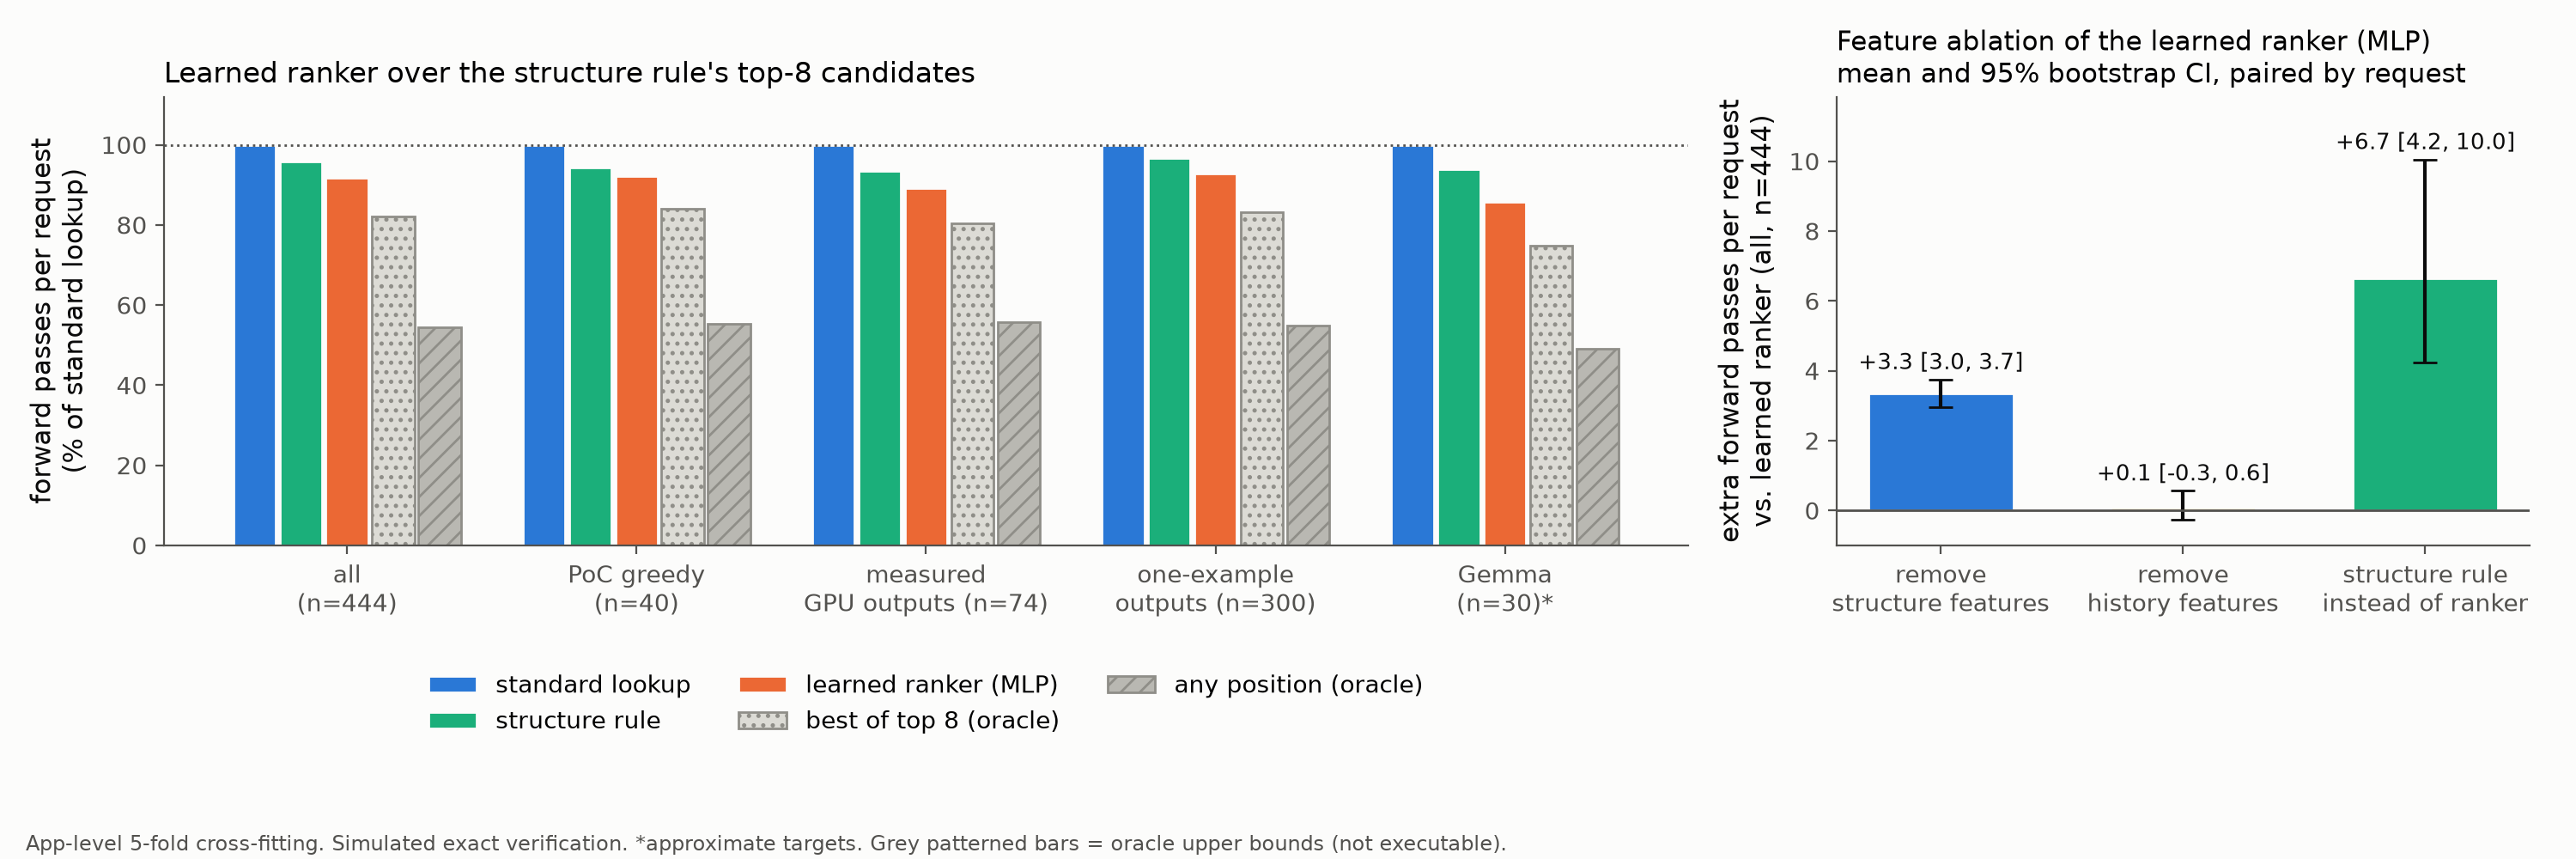
\includegraphics[width=\linewidth]{../runs/study/figures/ranker_paper.png}
\caption{Left: model passes in replay as a share of standard prompt lookup, lower is better, for several groups of recorded outputs. Grey patterned bars are upper bounds that use the future output. Right: extra passes when parts of the ranker are removed or replaced by the rule.}\label{fig:ranker}
\end{figure}

\section{Robustness and strong baselines}
\subsection{Changing the HTML style}
We rewrote the example pages in four ways that keep the screen pixel-identical: added line breaks and indentation, moved CSS rules into the elements, wrapped elements in extra invisible containers, and renamed CSS classes. The ranker was not retrained.

\begin{table}[H]\centering\small
\caption{Real time with rewritten examples, which the model then imitates; 50 requests, one repetition. Source: \texttt{POC\_method.md}, section 6.4.}\label{tab:p1}
\begin{tabular}{lll}
\toprule
rewrite & prompt lookup $-$ structure rule & structure rule $-$ learned ranker\\
\midrule
none & $+6.8\%$ $[+3.7, +9.9]$ & $+5.1\%$ $[+1.8, +8.1]$\\
line breaks and indentation & $+6.4\%$ $[+0.4, +12.7]$ & $-11.5\%$ $[-27.8, -1.1]$\\
CSS moved into elements & $+11.9\%$ $[+6.4, +16.8]$ & $0.0\%$ $[-6.9, +5.3]$\\
extra containers & $+6.9\%$ $[+4.2, +9.6]$ & $+3.7\%$ $[-0.9, +8.3]$\\
renamed classes & $+6.2\%$ $[+1.2, +10.7]$ & $+2.6\%$ $[-2.1, +6.6]$\\
\bottomrule
\end{tabular}
\end{table}
\textbf{Verified.} The rule stays significantly faster than prompt lookup under all four rewrites, and accuracy does not drop: the checklist stays between 89\% and 96\% for every rewrite and method. The ranker loses to the rule when line breaks are added and shows no clear difference otherwise. The cause is a shift in the model's own output: it also breaks the CSS into lines, which the examples do not do, so the average accepted draft falls from about 4 tokens to 1.5, and the ranker's inputs move far outside the range it was trained on. When only the draft source was rewritten and the model saw the original examples, the rule was faster than prompt lookup for three of the four rewrites in seconds, and the ranker did not fail.

\subsection{SuffixDecoding}
SuffixDecoding keeps two memories of text: one for the current request, and a global one built from the outputs of other requests. It drafts the continuation that most often followed the current ending. We reproduced it from its official source code; the main difference is a draft limit of 16 tokens, the default of its serving plugin, with a limit of 64 as a check. Its global memory holds outputs of other apps only, plus the current request's own output, as in the official code.

\begin{table}[H]\centering\small
\caption{Replay on 114 recorded outputs, model passes per request. ``Tuned'' lets drafts grow longer relative to the matched ending. Source: \texttt{POC\_study.md}, sections 12 to 15.}\label{tab:sd}
\begin{tabular}{lr}
\toprule
draft choice & passes\\
\midrule
standard prompt lookup & 134.2\\
structure rule / learned ranker & 126.0 / 121.8\\
SuffixDecoding, current request only & 153.0\\
SuffixDecoding, default / with our ranker & 108.1 / 107.5\\
SuffixDecoding, tuned / with our ranker & 94.3 / \textbf{91.4}\\
upper bound: best place in the current request & 74.5\\
upper bound: best place including other requests' outputs & 46.9\\
\bottomrule
\end{tabular}
\end{table}
\textbf{Verified in replay.}
\begin{itemize}[itemsep=1pt]
\item On their own, our rule and ranker are clearly behind SuffixDecoding. Its advantage comes from the global memory: using only the current request, it is worse than prompt lookup.
\item The global memory does not leak: no output of the same request or app, and no copy of the true output, was ever in it. Filling it in a realistic serving order raises SuffixDecoding to 103.0 passes, and removing the most common shared phrases to 102.0, but in both cases about 80\% of its gain over prompt lookup remains.
\item Our earlier guess that the shared formatting of our data inflates SuffixDecoding's advantage is not supported: with rewritten HTML styles its gain over prompt lookup stayed the same or grew, except when extra containers were added, where it fell from 20\% to 15\%.
\item Ranking SuffixDecoding's candidates with our ranker saves 2.9 passes per request $[2.25, 3.61]$, 3.1\%, in the tuned setting, and 0.96 $[0.40, 1.54]$ with a draft limit of 64. In the default setting the saving is 0.52 $[0.14, 0.89]$ and not significant on two of three data subsets. The element-tree features alone account for 1.0 to 1.7 passes, depending on the HTML style.
\end{itemize}
\textbf{Hypothesis, not yet tested.} The largest room left lies between SuffixDecoding, 94.3 passes, and the best place including other requests' outputs, 46.9. Searching places in the global memory by structure is our next direction. None of the SuffixDecoding results have been measured in real time yet.

\section{Limitations}
\begin{itemize}[itemsep=1pt]
\item Real-time results use one small model, 50 development and 100 test requests, and a single run on the test set; a second HTML source is still being evaluated.
\item Outputs equal normal generation only in exact arithmetic; in practice rounding makes about half of them differ slightly, without a significant change in length.
\item The ranker is not robust to changes in output formatting. The rule is.
\item Against SuffixDecoding our gain is 1 to 3\% in replay, and small or absent in its default setting.
\item The model ran in a 4-bit format that only approximates the official release.
\end{itemize}

\section{Conclusion}
For HTML, the place a draft is copied from matters. On top of the 11 times speed-up from known techniques, a learned ranker that reads the element tree is 5.9\% faster than a hand-written structure rule and 9.5\% faster than standard prompt lookup on apps it has never seen, with unchanged quality. The rule alone helps clearly on development requests and under style rewrites, but not significantly on the test set, and the ranker is fragile when the output formatting changes. SuffixDecoding, which reuses other requests' outputs, is stronger than both, and our structure features add only 1 to 3\% on top of it. Choosing places across other requests' outputs by structure is the most promising next step.

\end{document}
